\textbf{COLUNI 2022 -- Questão 03}\par\medskip Leia o texto a seguir para as questões 03 e 04.

\par

% COLUNI-AUTO-FIGURES-BEGIN
\begin{figure}[htbp]
\centering
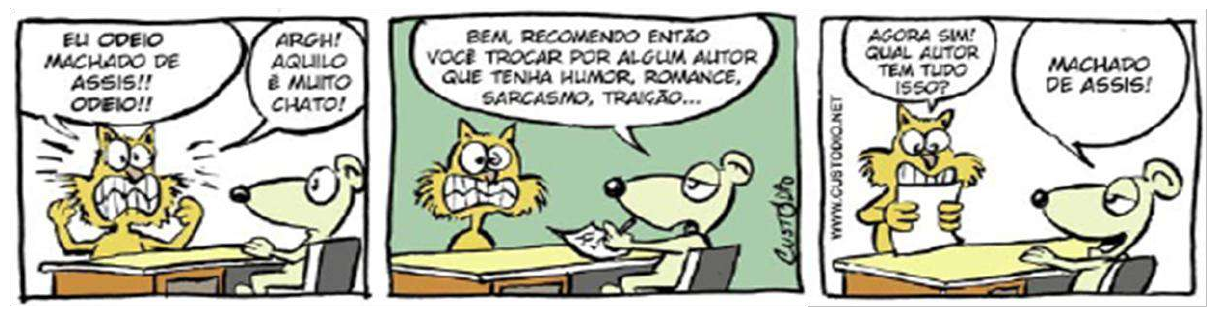
\includegraphics[width=0.95\linewidth]{static/simulados/coluni/figuras/2022/questao-03/figura-1.png}
\end{figure}
% COLUNI-AUTO-FIGURES-END

Disponível em: https://enem.estuda.com/questoes/?id=399426 tirinhas+de+literatura\&tbm=isch\&source. Acesso em: 31 ago. 2021.

\par

No diálogo da tirinha, a fala do personagem “rato”, ao recomendar a troca do autor:


\begin{enumerate}
\item zomba do personagem “gato”.
\item despreza o personagem “gato”.
\item repudia o personagem “gato”.
\item duvida do personagem “gato”.\end{enumerate}
